% 本科毕业论文选项
\documentclass[bachelor,fandolfonts,replaceperiod]{jnuthesis} 
% Font: winfonts, sourcefonts, adobefonts, fandolfonts
% modify colrlinks in ‘junthesis.cls’ at line 172
%\input{bachelor-common}
%\usepackage[math]{blindtext}
\usepackage[version=4]{mhchem}
\usepackage{zhlipsum}
\usepackage{lipsum}
%\usepackage{subfigure}
%\graphicspath{{Figure/}}
\titlea{含硒表面活性剂囊泡的构筑}
\titleb{与性质研究}
\author{陈育明}
\studentnum{1050115220}
\supervisor{刘雪锋}
\supervisorpos{教授}
\supervisorb{}
\supervisorbpos{}
\major{应用化学}
\department{化学与材料工程}
\institute{江南大学}
% 学士学位获得日期,需设置年、月,默认为编译日期。
\bachelordegreeyear{2019}
\bachelordegreemonth{6}

\begin{document}
    % 制作中文封面
    \maketitle
    % 开始前言部分
    \frontmatter
    % 论文的中文摘要
    \begin{abstract}
        复杂网络的研究可上溯到20世纪60年代对ER网络的研究。90年后代随着Internet
        的发展,以及对人类社会、通信网络、生物网络、社交网络等各领域研究的深入,
        发现了小世界网络和无尺度现象等普适现象与方法。对复杂网络的定性定量的科
        学理解和分析,已成为如今网络时代科学研究的一个重点课题。
        \keywords{开关表面活性剂;硒;氧化还原;囊泡}
    \end{abstract}
    
    % 论文的英文摘要
    \begin{englishabstract}
        \lipsum[1-2]
        % 英文关键词。关键词之间用英文半角逗号隔开,末尾无符号。
        \englishkeywords{Switchable Surfactant, Selenium, Redox, Vesicle}
    \end{englishabstract}
    
    % 生成论文目次
    \tableofcontents
    
    % 开始正文部分
    \mainmatter
    
    \chapter{绪论}\label{chapter:introduction}
    \section{引言}
    表面活性剂 (surfactant, surface active agent) 是一种能够溶于水且可使水的表(界)面张力显著降低的物质,
    传统上认为表面活性剂是在很低浓度下仍可显著降低液体表(界)面张力的物质,现在一般认为只要在较低
    浓度下可以显著改变表面性质的物质即可划归表面活性剂的范畴。
    
    表面活性剂分子一般由两部分构成:一部分为疏水(亲油)的非极性基团,通常为八个碳以上的烃链;另一
    部分为亲水的极性基团,例如羧基、羟基、磺酸基、季铵基等。表面活性剂分子既亲水又亲油,故被称为
    两亲分子,最典型的例子是肥皂,具有增溶、润湿等作用。表面活性剂因其乳化、润湿、增溶等优良作用而
    被广泛用于如原油回收、土壤修复、乳液聚合、药物制备等领域\cite{秦勇2009}。
    
    \section{刺激响应型表面活性剂}
    一般情况下,表面活性剂大多具有性能稳定的特点,但在大多数情况下,它只需在某一阶段起作用,之后反而
    会产生分离困难;另一方面,表面活性剂一般不参与化学反应,直接排放既是一种浪费,同时给环境带来压力
    \cite{秦勇2009}。因此先后发展了多样触发机制的可分解型表面活性剂 (cleavable surfactants) 和开关型表面
    活性剂 (switchable surfactants)。
    
    \subsection{可分解型表面活性剂}
    为应对传统表面活性剂生物降解速率慢及其引起的环境问题,人们开始关注于可分解表面活性剂,设想通过在
    分子内嵌入易断裂化学键以提高生物降解速率(尽管研究中的高效催化降解不完全代表实际中微生物也能够
    高效地降解)\cite{tehrani2007},此类可分解表面活性剂在酸碱、光照、加热、酶催化等条件下能够促发分解\cite{hellberg2000}。
    传统表面活性剂一般相对稳定,早在可分解表面活性剂的概念开始发展之前,季铵酯类表面活性剂早已被用作
    纺织品柔软剂,这便是典型的可分解表面活性剂。此外,十二烷基硫酸钠能够进行自催化降解、脂肪酸聚氧乙烯酯
    这一表面活性剂应当在中性或弱碱性条件下使用、羰基类表面活性剂在酸性条件会分解这些可分解表面活性剂
    的分解条件均被人们加以应用\cite{tehrani2007}。
    
    对于可分解表面活性剂,其催化分解的手段主要包括:酶、酸、碱、UV光照、臭氧以及加热等。可分解表面
    活性剂主要包含对酸不稳定类(缩醛类、缩酮类、原酸酯类及硅氧烷基表面活性剂)、对碱不稳定类(季铵酯、
    甜菜碱酯、单烷基(醚)碳酸酯)以及对UV-光照、热及臭氧不稳定的各类表面活性剂\cite{hellberg2000,tehrani2007,shukla2010,narayanan2008}。    
%        \begin{figure}
%            \centering
%            \begin{subfigure}[b]{\textwidth}
%                \centering
%                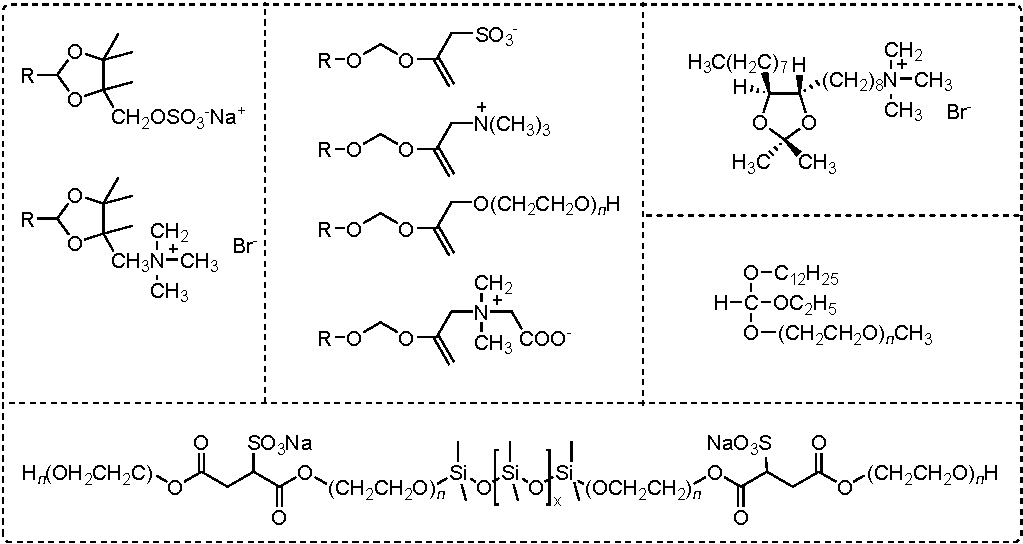
\includegraphics[width=\textwidth]{Figure/cleavable-a.pdf}
%                \caption{对酸性不稳定的可分解表面活性剂}\label{fig:cleavable-a}
%            \end{subfigure}%
%        
%            \begin{subfigure}[b]{\textwidth}
%                \centering
%                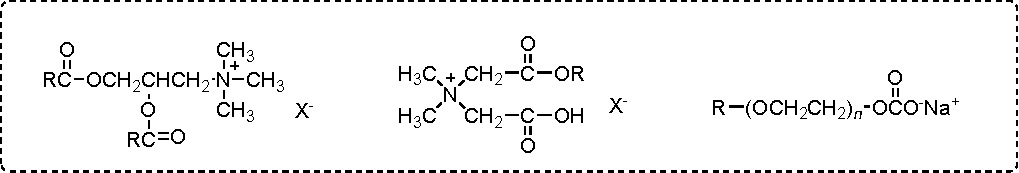
\includegraphics[width=\textwidth]{Figure/cleavable-b.pdf}
%                \caption{对碱性不稳定的可分解表面活性剂}\label{fig:cleavable-b}
%            \end{subfigure}%
%        
%            \begin{subfigure}[b]{\textwidth}
%                \centering
%                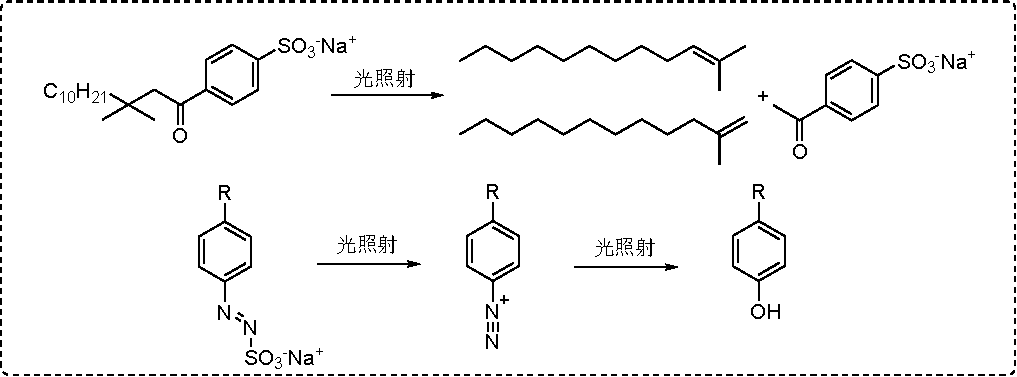
\includegraphics[width=\textwidth]{Figure/cleavable-c.pdf}
%                \caption{光照分解表面活性剂}\label{fig:cleavable-c}
%            \end{subfigure}%
%    
%            \begin{subfigure}[b]{\textwidth}
%                \centering
%                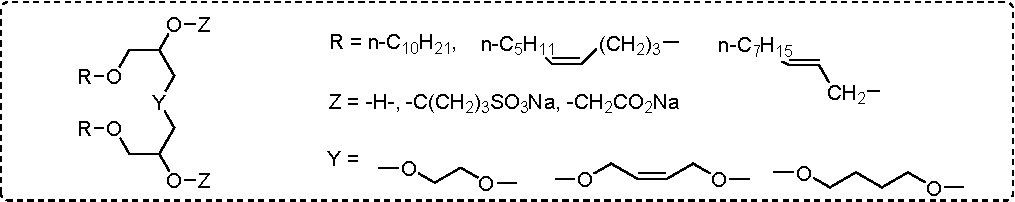
\includegraphics[width=\textwidth]{Figure/cleavable-d.pdf}
%                \caption{臭氧分解表面活性剂}\label{fig:cleavable-d}
%            \end{subfigure}%
%        \end{figure}

%        \begin{figure}[t]
%        \ContinuedFloat
%            \begin{subfigure}[b]{\textwidth}
%                \centering
%                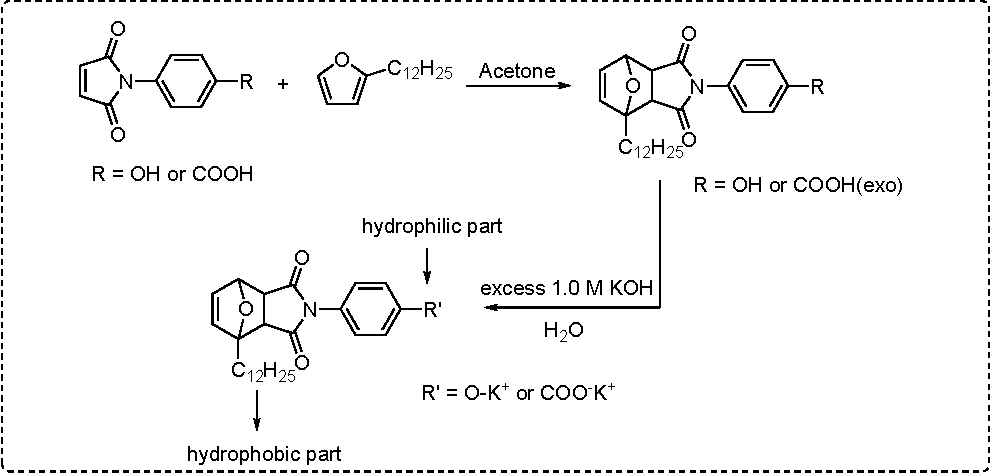
\includegraphics[width=\textwidth]{Figure/cleavable-e.pdf}
%                \caption{臭氧分解表面活性剂}\label{fig:cleavable-e}
%            \end{subfigure}%
%            \caption{已发展的可分解表面活性剂类型}\label{fig:cleavable-saa}
%        \end{figure}
    
    发展可分解表面活性剂最初是面向解决传统表面活性剂难以生物降解带来的环境问题,这一方面已有
    PPS、ProteaseMAX、RapiGest SF等商品化洗涤产品。此外,可分解型表面活性剂亦可用于用于乳液
    破乳、纳米粒子及聚合物制备的模板剂\cite{liu2007}、膜蛋白的质谱分析\cite{norris2003}及胶束电动
    色谱\cite{stanley2012}、囊泡药物装载及释放\cite{guo2012}等方面。但与此同时,化学或酶催化降解
    的可分解表面活性剂或是并不能完全适应于微生物降解\cite{tehrani2007},或是降解速率有待提高,
    更重要的是可分解表面活性剂的分解过程具有不可逆性\cite{liu2007}。
    
%    Liu等\cite{guo2012}以氯化肉豆蔻酰胆碱(及一种季铵酯表面活性剂,在酶催化或碱催化下可分解)及
%    对磺酸杯芳烃(SC4A)构建二级囊泡,利用氯化肉豆蔻酰胆碱在丁酰胆碱酯酶(BChE)作用下酯键
%    断裂,或可应用于阿尔茨海默症的载药及释放(见图\ref{fig:Ch1-SC4A})。
%    \begin{figure}[htbp]
%        \centering
%        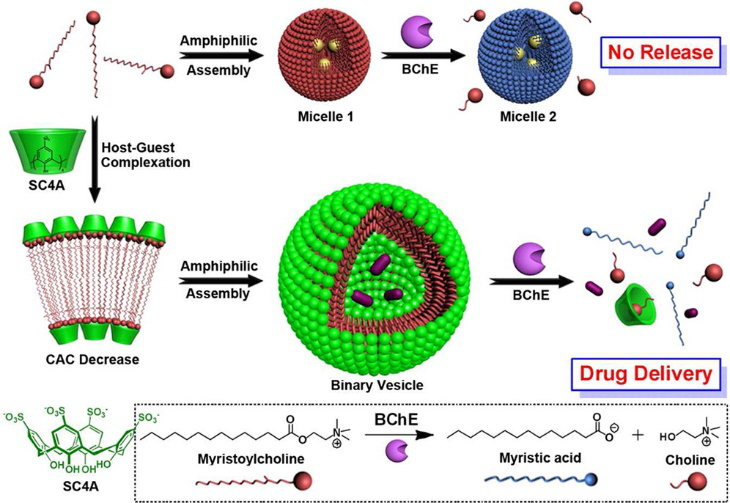
\includegraphics[width= 0.55\textwidth]{Figure/Ch1-SC4A}\\
%        \caption{肉豆蔻酰胆碱在SC4A空白及存在下的两亲自组装示意图}\label{fig:cleavale-SC4A}
%    \end{figure}
    
   \subsection{开关型表面活性剂}
    20世纪80年代以来,开始发展出各种触发机制的开关表面活性剂(switchable surfactants),
    用于可逆地调控表面活性剂性质。例如,需要聚合物乳胶悬浮液在储存运输过程中保持稳定,
    但当其被施工涂刷到物体表面之后,就需要对针对悬浮液“稳定”的性质进行“关闭”,这显然是
    开关表面活性剂的优点\cite{jessop2012},同时这种性质上的“关闭”是可以恢复的,这也是
    相较于可分解型表面活性剂的独到优势。例如,非离子表面活性剂就是一类传统的温度开关
    表面活性剂,当温度上升,其亲水性降低、表面活性降低,但当温度恢复时其性质亦恢复。
    根据这些刺激响应的方式,可以将开关表面活性剂分为:光开关、磁开关、温度开关、酸碱
    开关、\ce{CO2}开关以及氧化还原开关和酶开关表面活性剂\cite{秦勇2009}。
    
    \subsection*{(1) 光开关表面活性剂}
    光开关表面活性剂在非极性疏水尾链或极性亲水头基中具有适当的显色基团\cite{张冤帝2017}。
    根据所需光照条件可将光开关表面活性剂分为两类:一类是稳定型的,利用不同波长的光可
    调节表面活性剂的表面活性;另一类是不稳定的,只有用连续光照才能够实现其表面活性的转变。
    
    根据表面活性剂分子在转变中的变化特点,可以将光开关表面活性剂分为顺反异构型、裂解-聚合型
    以及极性变化型开关表面活性\cite{张冤帝2017,李云霞2011}。顺反异构型开关表面活性剂是
    研究较早的光开关表面活性剂,其主要结构有偶氮苯类、二苯乙烯类以及烷基苯乙烯衍生物等。
    异构型光开关表面活性剂的代表型结构见图\ref{fig:switchable-light}\cite{张冤帝2017,karthaus1996,shang2003,吕湘亮2018}。
    
    \begin{figure}[htbp]
        \centering
        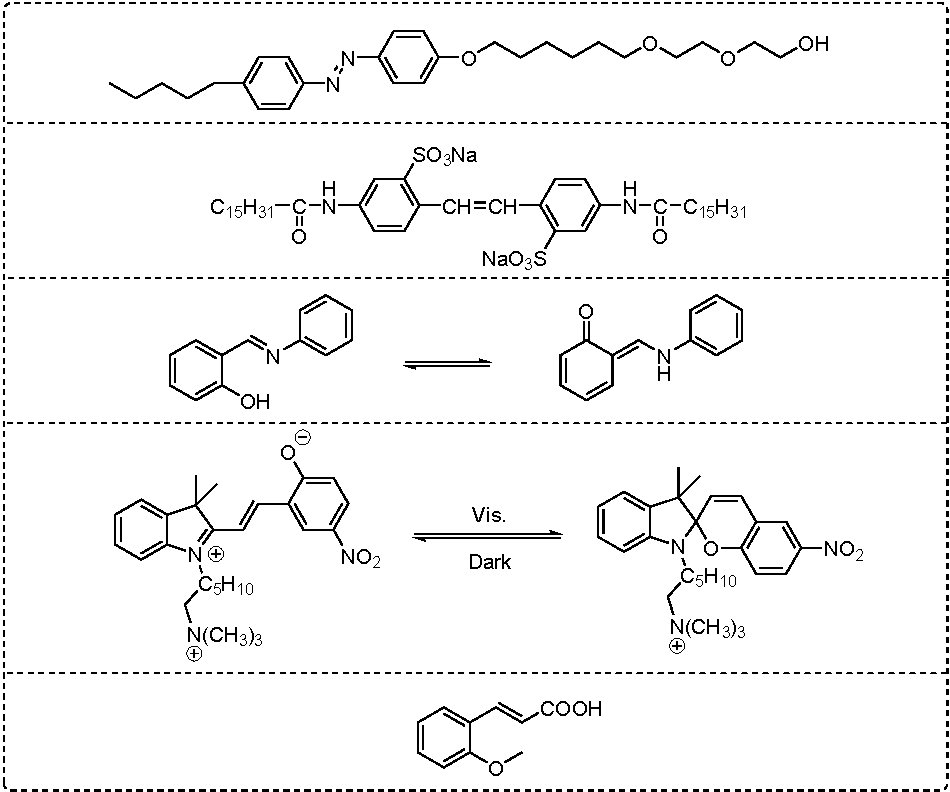
\includegraphics[scale=0.8]{Figure/switchable-light.pdf}\\
        \caption{异构型光开关表面活性剂代表结构\cite{张冤帝2017,karthaus1996,shang2003,吕湘亮2018}}\label{fig:switchable-light}
    \end{figure}
    
    其中,偶氮型光开关表面活性剂研究较早,应用较广,但是一些光敏型表面活性剂\cite{刘清斌2018}如偶氮类分解型及
    光照不可逆型的表面活性剂当属于刺激响应型表面活性剂,确切地分类应不属于开关型表面活性剂。刘清斌在其硕士论文中对光敏型表面活性剂做了总结。
    
    光开关表面活性剂在生物医药、环境修复及减阻传热等方面具有应用价值\cite{刘清斌2018},其中
    关于偶氮类光致异构化的表面活性剂研究较多,Chen等\cite{chen2016}采用偶氮类阳离子表面活性剂
    BTAEAzo实现绿色化的泡沫染整工艺。
    
    除光开关表面活性剂之外,还可以使用具有光刺激响应分子与表面活性剂作用,构成具有光刺激响应
    的体系。Zhao等\cite{zhao2016}将反式邻甲氧基肉桂酸与N-甲基-N-乙基吡咯烷溴化物(C16MPB)在
    碱性条件下自组装为粘弹性蠕虫状胶束,经UV光照后反式邻甲氧基肉桂酸构型转变,从而使体系转变
    成球形或棒状胶束,见图\ref{fig:switchable-light-omca}。
    
    \begin{figure}[htbp]
        \centering
        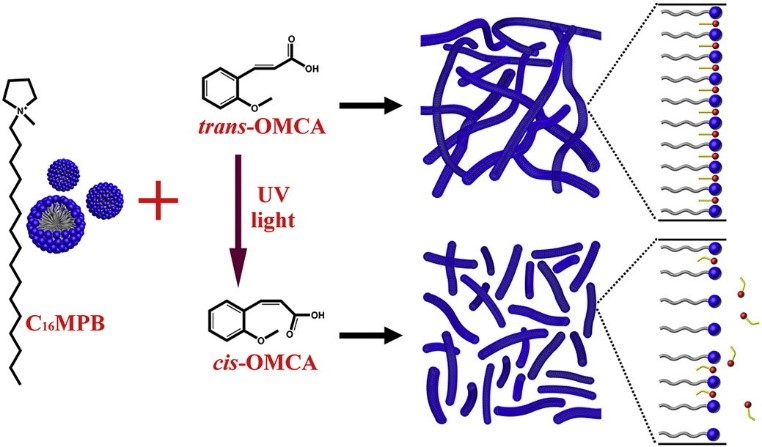
\includegraphics[width=.7\textwidth]{figure/switchable-light-omca.jpg}\\
        \caption{N-甲基-N-乙基吡咯烷溴化物 (C16MPB) 与邻甲氧基肉桂酸构建的光刺激响应性体系\cite{zhao2016}}
        \label{fig:switchable-light-omca}
    \end{figure}
        
    \subsection*{(2) 磁开关表面活性剂}
    磁开关表面活性剂主要为含有磁响应结构,包含离子液体、螯合型以及多金属氧酸盐表面活性剂,
    此外,磁性有机分子表面活性剂是有待发展的新一类磁表面活性剂\cite{brown2015},磁响应表面
    活性剂可用于蛋白质分离、水处理以及环境修复\cite{brown2015}等方面。主要类别磁响应表面活
    性剂见图\ref{fig:switchable-mag}。
    \begin{figure}[htbp]
        \centering
        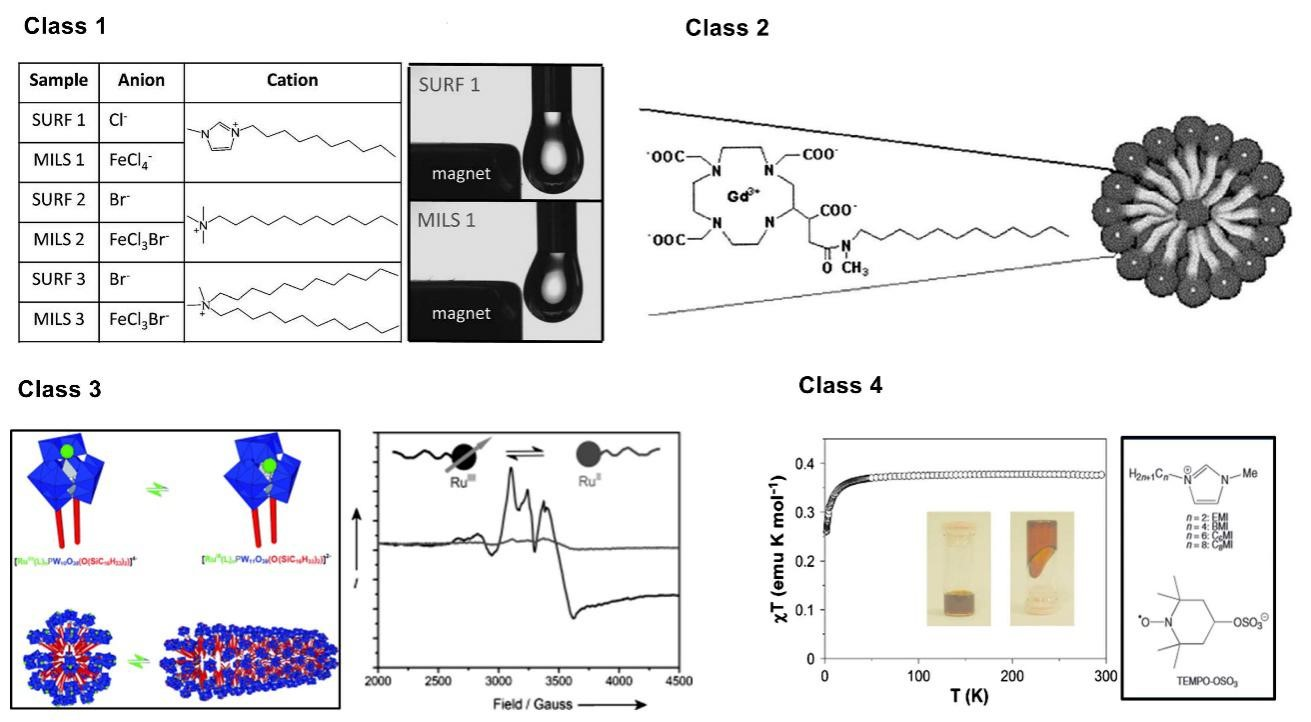
\includegraphics[width=.985\textwidth]{figure/switchable-mag.jpg}\\
        \caption{主要类别的磁开关表面活性剂\cite{brown2015,brown2012}}
        \label{fig:switchable-mag}
    \end{figure}
    
    \subsection*{(3) 温度开关表面活性剂}
    非离子型表面活性剂是典型的温度开关表面活性剂,随温度升高其亲水性会逐渐下降,至浊点时其
    亲水性显著降低,表面活性变差,而当温度降低后其又可恢复表面活性。Chu\cite{chu2011}等以
    棕榈酰氨基磺基甜菜碱 (PDAS) 为表面活性剂制备了一种具有温度响应的凝胶,在 30 ℃ 时形成
    球状或短棒状胶束,在 40 ℃ 时则形成网络蠕虫状胶束\ref{fig:switchable-temperature},这是由于加热时疏水部分溶解度降低,
    从而形成网状交联凝胶。
    \begin{figure}[htbp]
        \centering
        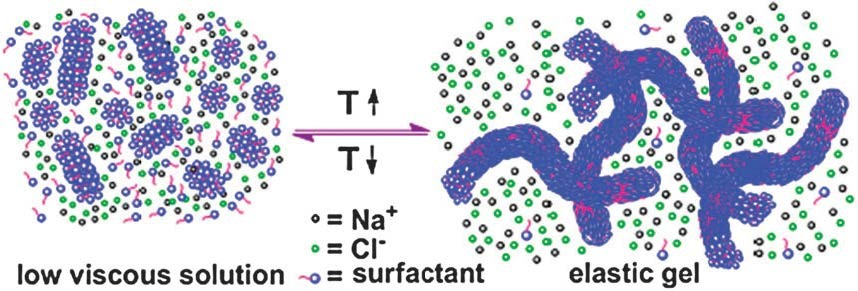
\includegraphics[width=.711\textwidth]{figure/switchable-temperature.jpg}\\
        \caption{应用温度开关表面活性剂的可转换温感凝胶\cite{chu2011}}
        \label{fig:switchable-temperature}
    \end{figure}

    \subsection*{(4) 酸碱开关表面活性剂}
    酸碱开关表面活性剂,亦即 pH 开关表面活性剂,此类表面活性剂通常含有羧酸、脒基、
    胍基等酸性或碱性基团,在 pH 发生变化时,这些基团接受或给予质子,导致表面活性剂的
    亲疏水性发生变化,从而调控表面活性剂的表面活性\cite{吕湘亮2018}。Lv等\cite{lv2014}
    合成了一类酸碱开关 Gemini 表面活性剂,通过调控 pH 可实现制备的乳液在O/W乳液和
    W/O乳液之间转变,图\ref{fig:switchable-ph}。
    \begin{figure}[htbp]
        \centering
        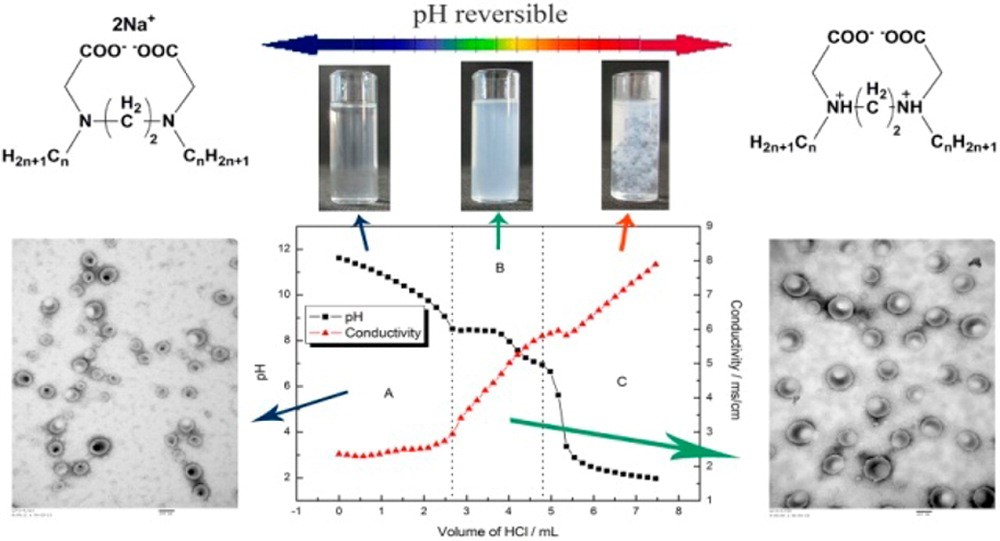
\includegraphics[width=.87\textwidth]{figure/switchable-ph.jpg}\\
        \caption{pH开关表面活性剂控制的乳液类型转变\cite{lv2014}}
        \label{fig:switchable-ph}
    \end{figure}

    除通过pH调节表面活性剂的亲疏水性改变体系性质外,Brazdova\cite{李云霞2011,brazdova2008}等
    制得脂质体表面活性剂,通过 pH 控制分子构象发生转换作为开关,见图\ref{fig:switchable-ph-conformation}。
    \begin{figure}[htbp]
        \centering
        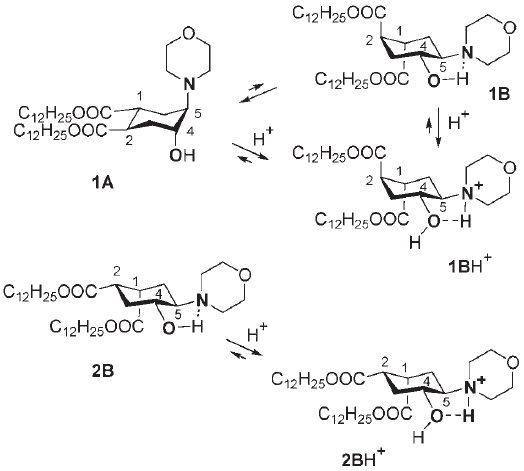
\includegraphics[width=.55\textwidth]{figure/switchable-ph-conformation.png}\\
        \caption{pH 触发的氨基环己醇衍生脂质构象变化\cite{brazdova2008}}
        \label{fig:switchable-ph-conformation}
    \end{figure}

    \subsection*{(5) \ce{CO2}/\ce{N2}开关表面活性剂}
    \ce{CO2}型开关表面活性剂其作用原理在本质上和酸碱开关表面活性剂类似,利用\ce{CO2}
    气体的弱酸性,随着\ce{CO2}的通入和排出,体系的 pH 发生变化,从而引起体系内可离子化基团的
    质子化或去质子化,导致表面活性剂亲疏水性发生变化,进而影响体系的表面活性。迄今为止,
    \ce{CO2}开关型表面活性剂主要包括脒/\ce{CO2}体系、胍/\ce{CO2}体系以及胺/\ce{CO2}体系\cite{梅平2016}。
    
    \ce{CO2}型开关表面活性剂采用\ce{CO2}作为调控手段,相比其他调控手段而言,具有价格便宜、
    无毒无害且易于脱除等优点\cite{jessop2012},可应用于重油输送、土壤清洗、油砂分离及乳化
    聚合\cite{jessop2012}。同可分解表面活性剂一样,早在开关表面活性剂概念提出之前,\ce{CO2}型
    开关表面活性剂已投入使用,Moore 和 Lefevre 采用\ce{CO2}作为丁二烯/苯乙烯乳液聚合的开关表面
    活性剂,见图\ref{fig:switchable-co2-a},其中式左化合物具有乳化作用而式右化合物不具有乳化作用。
    \begin{figure}
    \centering
        \begin{subfigure}[b]{\textwidth}
            \centering
            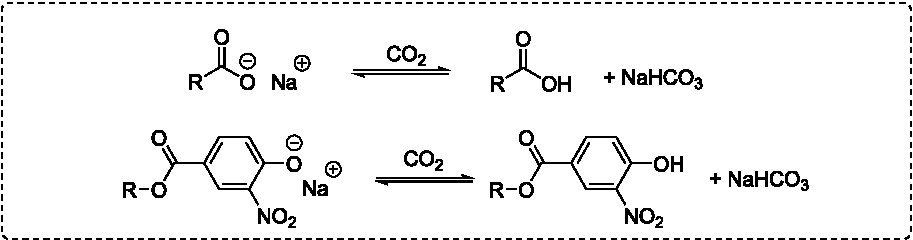
\includegraphics[width=\textwidth]{Figure/switchable-co2-a.pdf}
            \caption{Moore和Lefevre采用的丁二烯/苯乙烯乳液聚合可调控乳化剂}\label{fig:switchable-co2-a}
        \end{subfigure}%
    
        \begin{subfigure}[b]{\textwidth}
            \centering
            
\includegraphics[width=\textwidth]{Figure/switchable-co2-b.pdf}
            \caption{Jessop课题组提出的\ce{CO2}开关表面活性剂}\label{fig:switchable-co2-b}
        \end{subfigure}%
    \caption{早期应用及研究的\ce{CO2}型开关表面活性剂}
    \label{fig:switchable-co2}
    \end{figure}
    
    2006年,Jessop课题组\cite{liu2006science}提出一类脒类化合物可用于\ce{CO2}开关表面活性剂,
    见图\ref{fig:switchable-co2-b}。此外,三级胺也可用于\ce{CO2}开关表面活性剂,但一级、二级胺
    则因为形成氨基甲酸酯在开关表面活性剂应用中有所难度\cite{jessop2012}。
    
    \subsection*{(6) 氧化还原开关表面活性剂}
    氧化还原型开关表面活性剂主要采用电化学方法或化学手段改变表面活性剂分子结构,从而达到
    调整表面活性的目的。其中,前者研究最早且较为成熟的是二茂铁基表面活性剂,其包含阳离子-两性离子
    可逆转换和阴离子-两性离子可逆转换两类\cite{李云霞2011}。图\ref{fig:switchable-redox-cp2fe}中前者是
    一类二茂铁基表面活性剂。但二茂铁基开关表面活性剂所需使用的二茂铁基团价格对该类表面活性剂的广泛
    使用有所限制。
    \begin{figure}[htbp]
        \centering
        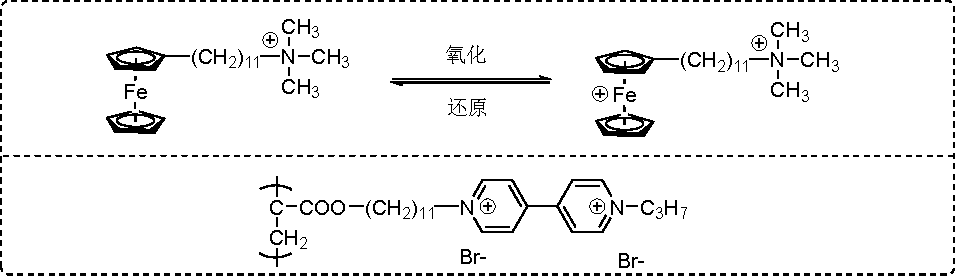
\includegraphics[width= \textwidth]{Figure/switchable-cp2fe.pdf}\\
        \caption{电化学方法实现 的氧化还原开关表面活性剂}\label{fig:switchable-redox-cp2fe}
    \end{figure}
    
    此外,甲基紫类结构,即联吡啶类结构的表面活性剂也是一类良好的氧化还原型开关表面活性剂,
    但此类表面活性剂毒性高,如氯化二甲基联吡啶(即百草枯主要成分,一种高毒植物农药)。
    
    除电化学方法实现的氧化还原开关表面活性剂外,含二硫键结构的表面活性剂可在含巯基试剂作用下断裂,
    从而改变分子结构。
    
%    最后,含硒表面活性剂作为一种新型的氧化-还原开关表面活性剂,Kong等\cite{kong2016redox}利用
%    \ce{H2O2}将硒醚氧化为硒亚砜,使尾链亲水性增加,且在\ce{Na2SO3}等还原条件下又可恢复原结构。
%    
%    图 13 含硒氧化-还原表面活性剂的可逆转化\cite{kong2016redox}
    
%    \subsection*{(7) 酶开关表面活性剂}
%    除以上类型的开关表面活性剂之外,还有酶催化\cite{ku2011}
%【Enzyme-triggered model self-assembly in surfactant–cyclodextrin systems】的开关表面活性剂有待讨论。
    
    
    \section{含硒表面活性剂}
    
    \section{囊泡}
    
    
    \section{论文的目的与创新}
    \subsection{研究目的}
    \subsection{创新之处}
    \subsection{研究内容}
    
    %%%%%%%%%%%%%%%%%%%%%%%%%%%%%%%%%%%%%%%%%%%%%%%%%%%%%%%%%%%%%%%%%%%%%%%%%%%%%%%
    \chapter{实验部分}\label{chapter:experiment}
    \section{实验仪器与试剂}
        \begin{table}[htp]
        \centering
        \begin{tabular}{ccc}
            \toprule
            \textbf{仪器/试剂} & \textbf{规格/型号} & \textbf{生产厂家} \\
            \midrule
            硒   & GR & 阿达玛斯试剂 \\
            硼氢化钠  & AR  & 上海化学试剂有限公司 \\
            1-溴代十二烷
            1-溴代丁烷  & CP & 国药集团化学试剂有限公司 \\
            3-溴丙醇 & GR & 阿达玛斯试剂 \\
            11-溴-1-十一醇 & ?? & 国药集团化学试剂有限公司 \\
            氯磺酸  & CP & 上海化学试剂有限公司 \\
            碳酸钠  & ?? & 国药集团化学试剂有限公司 \\
            十二烷基三甲基溴化铵 & ?? & 国药集团化学试剂有限公司\\
            30\%过氧化氢  & AR & 上海化学试剂有限公司 \\
            亚硫酸钠  & AR & 国药集团化学试剂有限公司 \\
            硫酸钠  & AR & 国药集团化学试剂有限公司 \\
            超纯水 & Simplicity\ce{^{\textregistered}} UV & 美国Merck Millipore\\
            电子分析天平  & JY2015 & 梅特勒-托利多有限公司 \\
            旋转蒸发器  & RE-2000B & 上海亚荣生化仪器厂 \\
            超声波清洗器  & KQ-100B & 昆山市超声仪器有限公司 \\
            超级恒温水浴  & ?? & 国药集团化学试剂有限公司 \\
            核磁共振谱仪  & AVANCE Ⅲ HD 400MHz & 瑞士布鲁克公司 \\
            液相色谱质谱联用仪  & LCZ/2690 XE/996 & 美国沃特世公司 \\
            激光光散射仪 & ALV/DLS/SLS-5022F & 德国ALV公司\\
            \bottomrule
        \end{tabular}
        \caption{实验仪器与试剂}\label{table:实验仪器与试剂}
    \end{table}

    \zhlipsum[1]
    
    \section{含硒表面活性剂的制备}
    \subsection{合成路线}
    采用图\ref{fig:synthesis-scheme}所示合成路线制备含硒表面活性剂3-十二烷基硒-1-丙基硫酸钠(SDSePS)和
    11-丁基硒-1-十一烷基硫酸钠(SBSeUS)。
    \begin{figure}[htbp]
        \centering
        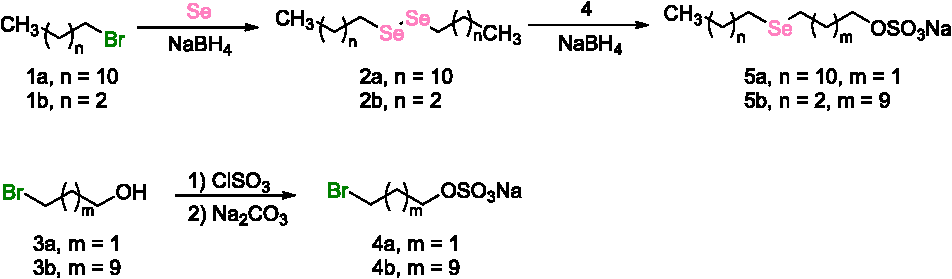
\includegraphics[scale=0.89]{figure/synthesis-scheme.pdf}\\
        \caption{含硒表面活性剂的合成路线}\label{fig:synthesis-scheme}
    \end{figure}
    \subsection{实验方法}
    \zhlipsum[1]
    
    \section{囊泡的构筑}
    \zhlipsum[1]
    
    \section{囊泡的性质研究}
    \subsection{不同摩尔比}
    
    \subsection{稳定性}
    
    \subsection{不同浓度}
    
    \subsection{氧化还原响应}
    
    \begin{definition}[平均路径长度]
        网络的平均路径长度$L$定义为任意两个节点之间的距离的平均值,即
        \begin{equation}\label{eq:avarage_path_lentgh}
        L = \frac{2}{N(N+1)}\sum_{i\geq j}d_{ij}
        \end{equation}
        其中$N$为网络节点数。网络的平均路径长度也称为网络的特征路径长度。
    \end{definition}
    
   %%%%%%%%%%%%%%%%%%%%%%%%%%%%%%%%%%%%%%%%%%%%%%%%%%%%%%%%%%%%%%%%%%
    \chapter{实验结果与讨论}\label{chapter:results}
    \section{含硒表面活性剂的表征与分析}
    \subsection{SDSePS的结构表征与分析}
    以\ce{CD3OD} (δ = 3.31)为溶剂,其中含有少量的\ce{H2O} (δ = 4.87)\cite{babij2016nmr} ,对纯化后的样品进行
    \ce{^1H} NMR 表征,表征与分析结果如图\ref{fig:NMR-12+3}所示。
    \begin{figure}[htbp]
        \centering
        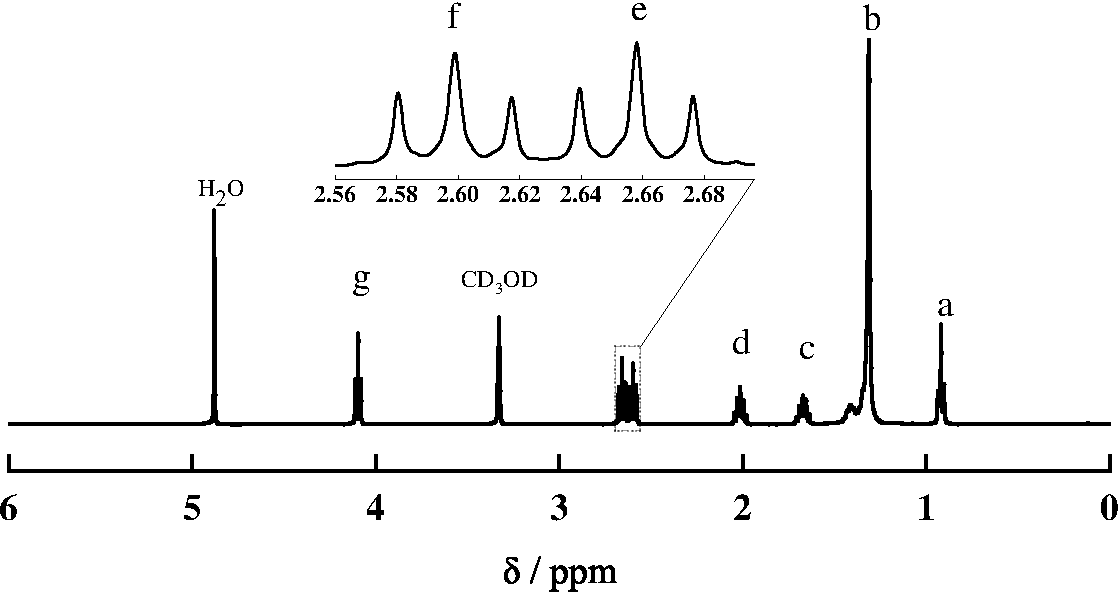
\includegraphics[width=.75\textwidth]{figure/nmr123.pdf}\\
        \caption{SDSePS的核磁氢谱}\label{fig:NMR-12+3}
    \end{figure}
     
    \ce{^1H} NMR (400 MHz, \ce{CD3OD}, 图\ref{fig:NMR-12+3}) δ 0.92 (t, \textit{J}=8.0 Hz, 3H), 1.31-1.41 (overlap, 18H), 1.67 (m, 2H), 2.01 (m, 2H), 2.60 (t, \textit{J}=8.0 Hz, 2H), 2.66 (t, \textit{J}=8.0 Hz, 2H),  4.10 (t, \textit{J}=6.0 Hz, 2H).
    
    对 \ce{C12SeAS} 的核磁共振氢谱进行解析,化学位移为 0.921 处的三重峰为 C12SeAS 疏水尾
    链端的甲基上的氢信号,以其积分个数为 3 计算,结果如表 2-5 所示,实际总氢个数为 31.68,
    理论氢个数为 31,氢个数基本吻合;如图 2-7 所示,e 处的两个三重峰氢信号为 Se 两端的亚
    甲基的氢信号,f 处亚甲基上的氢由于靠近极性头基(SO4 - ),出峰位置移动到 4.097,各个氢信
    号的出峰位置与目标产物能够对应,由此推断检测样品即为目标产物。
     \begin{figure}[H]
        \centering
        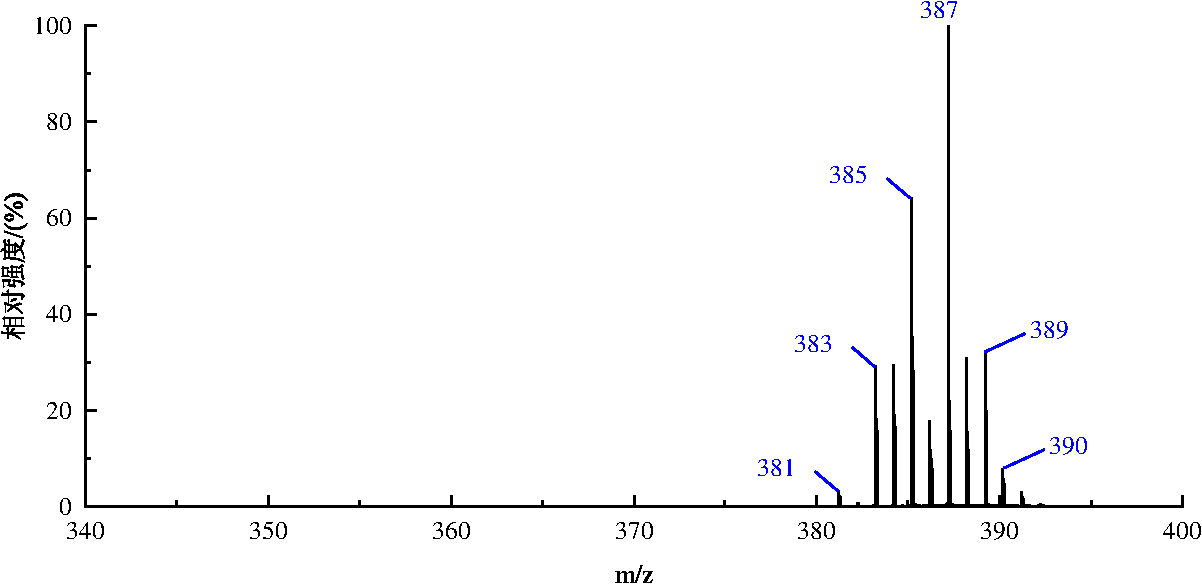
\includegraphics[width=.8\textwidth]{figure/mass123.pdf}\\
        \caption{SDSePS的质谱}\label{fig:mass-12+3}
    \end{figure}

HR-ESI-MS m/z 290.1422 [M – H] – (calcd 386.43 for \ce{C15H31SO4Se}).
%    \begin{figure}[htbp]
%    \centering
%        \begin{subfigure}[b]{.475\textwidth}
%            \centering
%            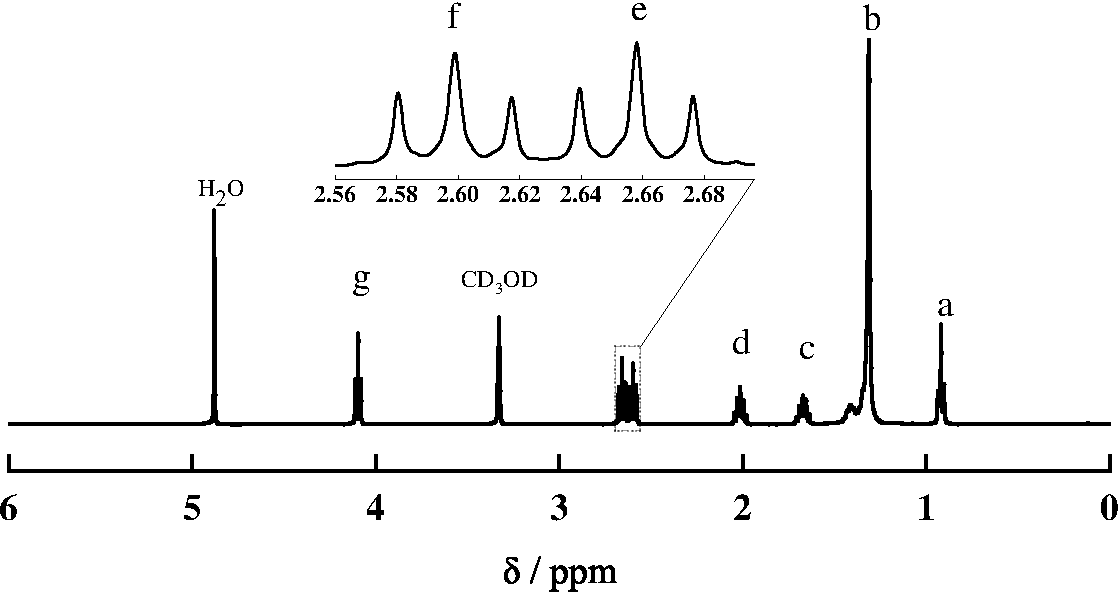
\includegraphics[width=\textwidth]{figure/nmr123.pdf}
%            \caption{核磁}\label{}
%        \end{subfigure}
%        \hfill
%        \begin{subfigure}[b]{.475\textwidth}
%            \centering
%            \includegraphics[width=\textwidth]{example-image}
%            \caption{质谱}\label{}
%        \end{subfigure}
%    \caption{12+3结构表征}\label{fig:cleavable-saa}
%    \end{figure}
%
%    \begin{figure}[htbp]
%        \centering
%        \begin{subfigure}[b]{.475\textwidth}
%            \centering
%            \includegraphics[width=\textwidth]{example-image}
%            \caption{核磁}\label{}
%        \end{subfigure}
%        \hfill
%        \begin{subfigure}[b]{.475\textwidth}
%            \centering
%            \includegraphics[width=\textwidth]{example-image}
%            \caption{质谱}\label{}
%        \end{subfigure}
%        \caption{4+11结构表征}\label{fig:cleavable-saa}
%    \end{figure}
    
    \subsection{SBSeUS的结构表征与分析}
        以\ce{CD3OD} (δ = 3.31)为溶剂,其中含有少量的\ce{H2O} (δ = 4.87)\cite{babij2016nmr} ,对纯化后的样品进行
    \ce{^1H} NMR 表征,表征与分析结果如图\ref{fig:NMR-12+3}所示。
    \begin{figure}[htbp]
        \centering
        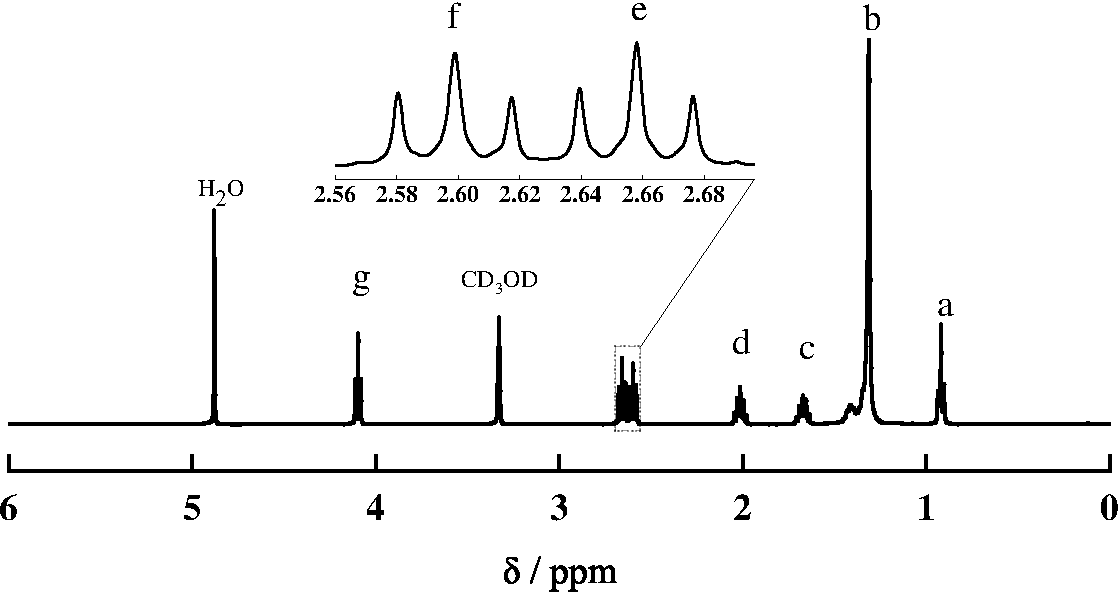
\includegraphics[width=.75\textwidth]{figure/nmr123.pdf}\\
        \caption{核磁}\label{fig:NMR-4+11}
    \end{figure}
    
    对 \ce{SDSePS} 的核磁共振氢谱进行解析,化学位移为 0.921 处的三重峰为 C12SeAS 疏水尾
    链端的甲基上的氢信号,以其积分个数为 3 计算,结果如表 2-5 所示,实际总氢个数为 31.68,
    理论氢个数为 31,氢个数基本吻合;如图 2-7 所示,e 处的两个三重峰氢信号为 Se 两端的亚
    甲基的氢信号,f 处亚甲基上的氢由于靠近极性头基(SO4 - ),出峰位置移动到 4.097,各个氢信
    号的出峰位置与目标产物能够对应,由此推断检测样品即为目标产物。
    \begin{figure}[htbp]
        \centering
        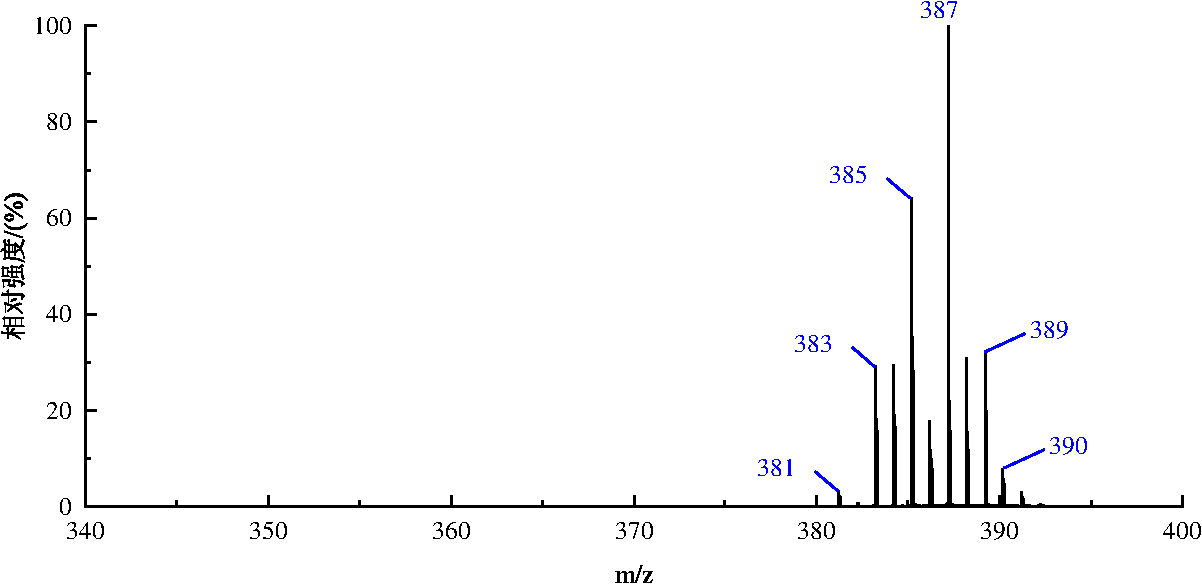
\includegraphics[width=.8\textwidth]{figure/mass123.pdf}\\
        \caption{质谱}\label{fig:mass-4+11}
    \end{figure}

    \section{阴阳离子表面活性剂囊泡的性质}
    \section{12+3复配囊泡的性质研究}
    \subsection{不同摩尔比复配}
    
    \subsection{囊泡稳定性}
    \begin{figure}[htbp]
        \centering
        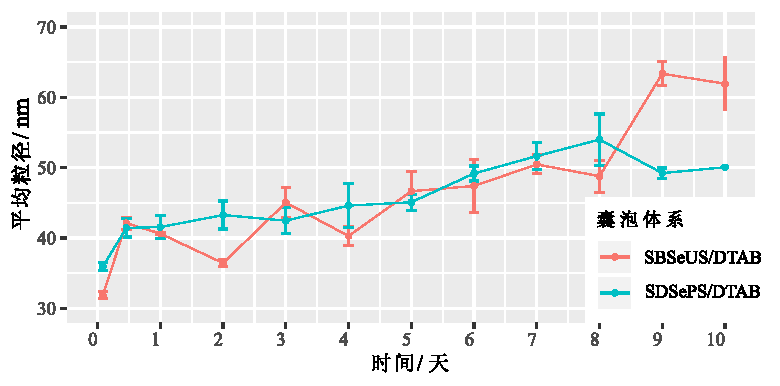
\includegraphics[width=0.95\textwidth]{figure/time.pdf}\\
        \caption{12+3不同浓度复配囊泡}\label{fig:ve}
    \end{figure}
    \subsection{不同浓度构筑含硒SAA囊泡}

    \begin{figure}[htbp]
        \centering
        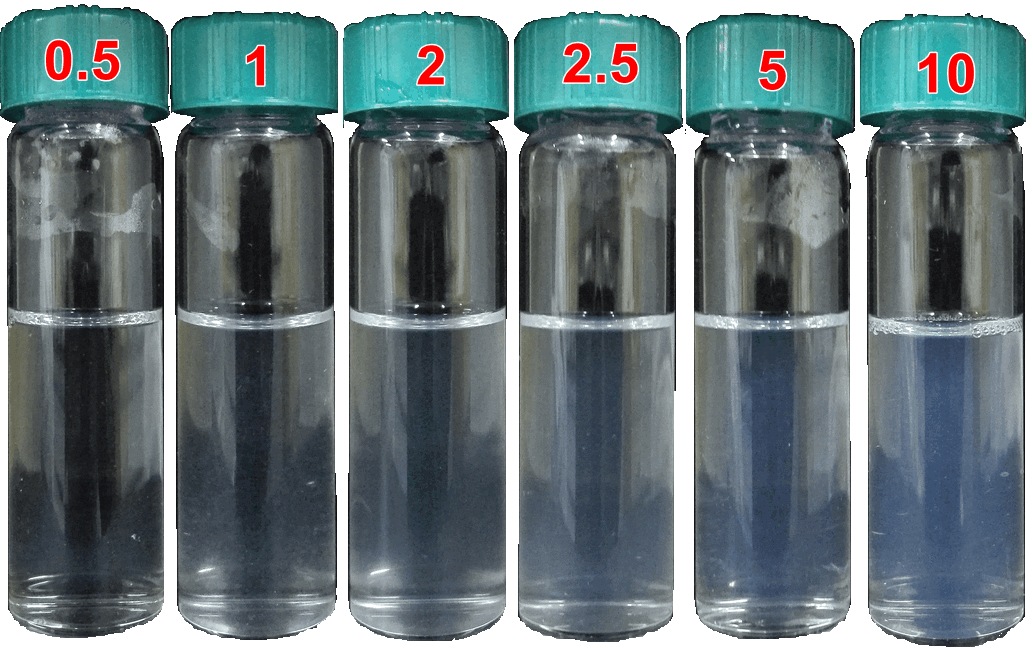
\includegraphics[height=4.5cm]{figure/123concentration.png}\\
        \caption{12+3不同浓度复配囊泡}\label{fig:vesicle-concentration}
    \end{figure}

    \begin{figure}[htbp]
        \centering
        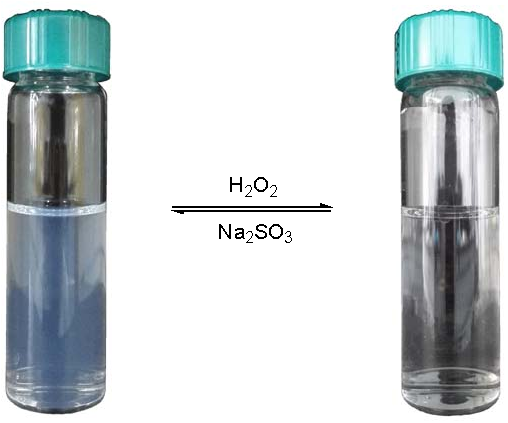
\includegraphics[height=4.5cm]{figure/redox.pdf}\\
        \caption{不同浓度复配囊泡}\label{fig:vesicle-redox}
    \end{figure}

    \subsection{氧化还原响应}
    
    
    [12+3]与DTAB复配囊泡
    
    \section{4+11复配囊泡的性质研究}
    \subsection{不同摩尔比复配}
        \begin{figure}[htbp]
        \centering
        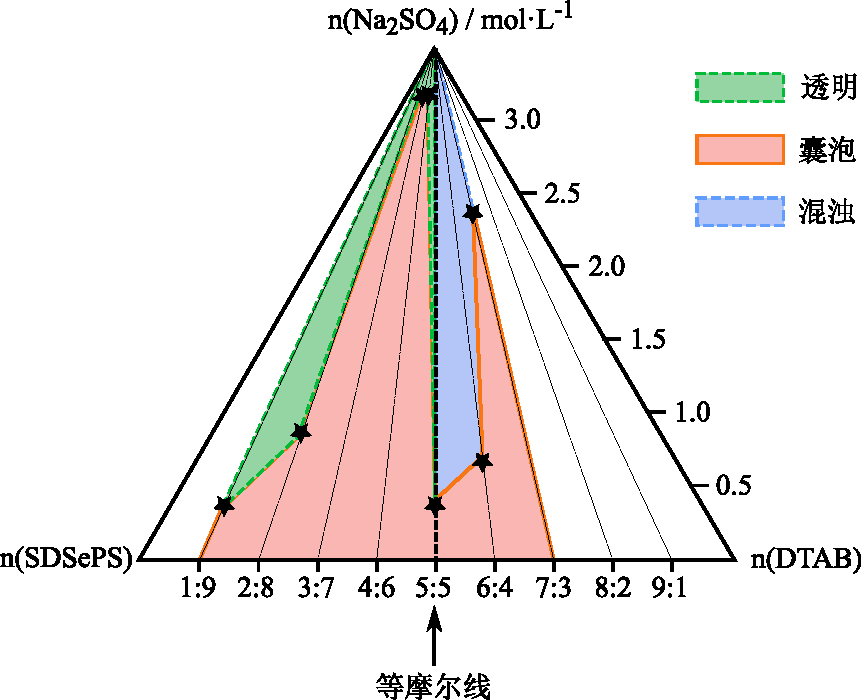
\includegraphics[width=0.52\linewidth]{figure/SDSePS-salt.pdf}\\
        \caption{SBSeUS/DTAB囊泡示意图}\label{fig:SDSePS-salt}
    \end{figure}

        \begin{figure}[htbp]
    \centering
    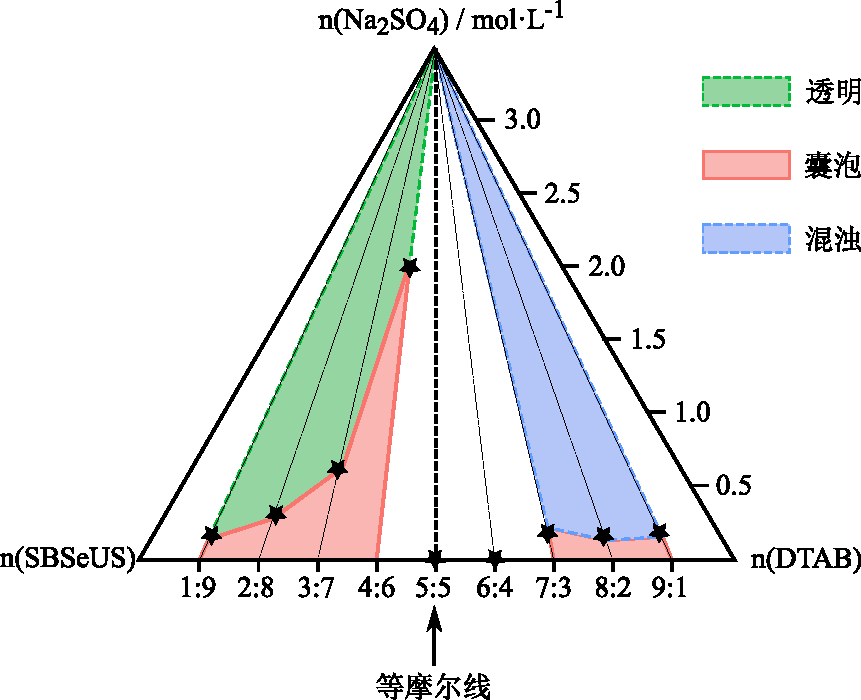
\includegraphics[width=0.52\linewidth]{figure/SBSeUS-salt.pdf}\\
    \caption{SBSeUS/DTAB囊泡示意图}\label{fig:SBSeUS-salt}
\end{figure}
    \subsection{囊泡稳定性}
    
    \subsection{不同浓度}
    \begin{figure}[htbp]
        \centering
        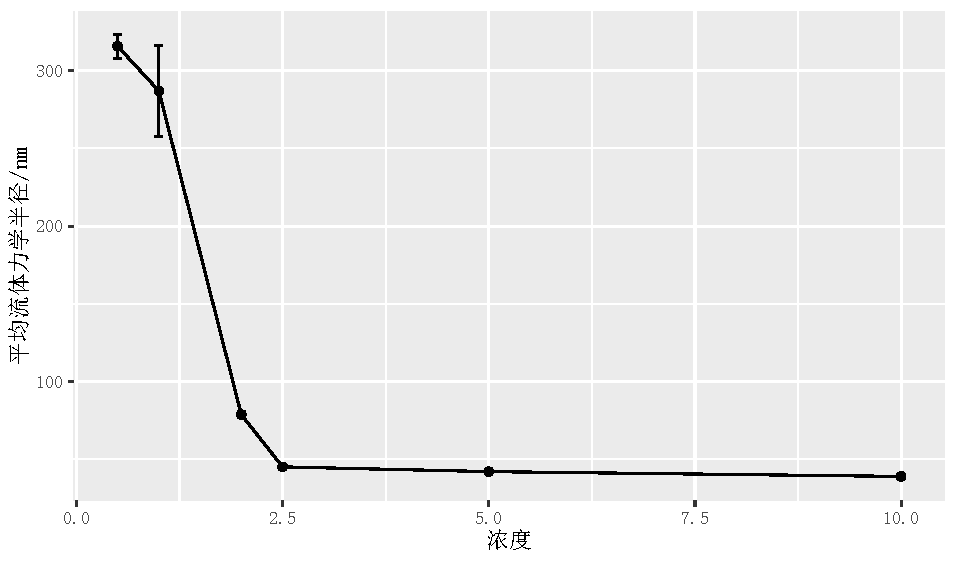
\includegraphics[]{Figure/test.pdf}\\
        \caption{4+11不同浓度复配囊泡}\label{fig:vesicle-concentration-line}
    \end{figure}
    \subsection{氧化还原响应}
    
    \begin{figure}[htbp]
        \centering
        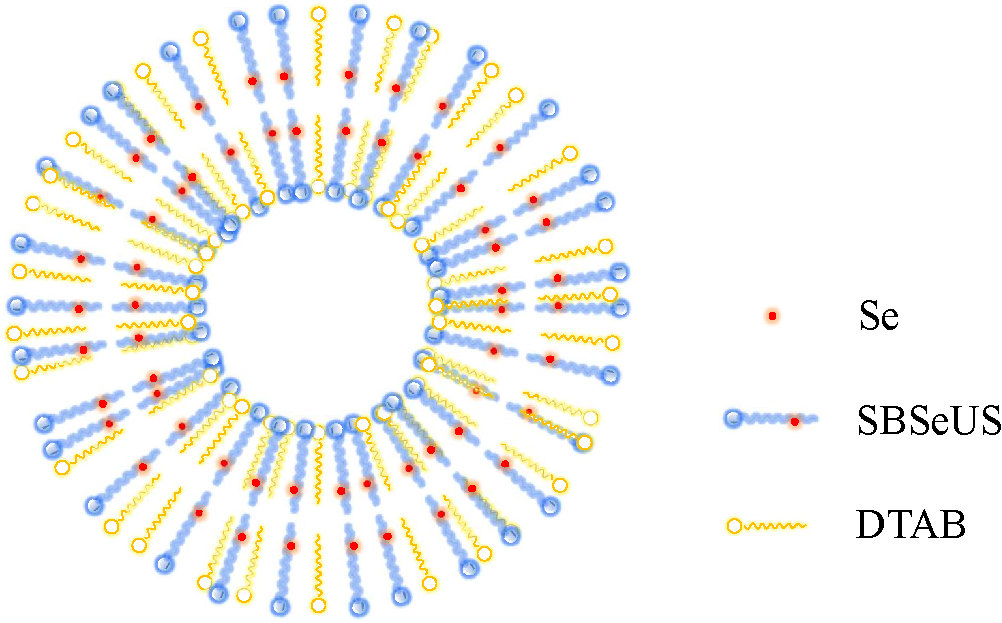
\includegraphics[width=0.46\linewidth]{figure/vesicle-scheme.pdf}\\
        \caption{SBSeUS/DTAB囊泡示意图}\label{fig:vesicle-concentration-line}
    \end{figure}
    [一次还原稳定性]加入后立即
    \section{本章小结}

    %%%%%%%%%%%%%%%%%%%%%%%%%%%%%%%%%%%%%%%%%%%%%%%%%%%%%%%%%%%%%%%
    % 学位论文的正文应以《结论》作为最后一章
    \chapter{结论与展望}\label{chapter:concludes}
    \section{结论}
    本文在第\ref{chapter:experiment}章中,通过考虑数据中心网络布局构建中的最大度限制
    问题,提出了符合数据中心网络基本要求的DS小世界模型,并分析了它的性质。随后提出
    SIDN,将DS模型映射到具体的网络结构中,并分析了所构成网络的平均直径、网络总带宽、
    对故障的容错能力等各项网络性能。
    
    \zhlipsum[1-3]
    
    \section{不足之处及未来展望}
    在第\ref{chapter_experiments}章中,针对网络模型研究这一类工作的共性,设计构造通
    用验证平台系统。以海量虚拟机和虚拟分布式交换机的形式,实现了基于少量物理节点,对
    大规模节点的模拟。其模拟运行的过程与真实运行在实现层面完全一致,运行的结果与真实
    环境线性相关。除为本文所涉若干网络模型提供验证外,可进一步推广到更为广泛的领域,
    为各种网络模型及路由算法的研究工作,提供分析、指导与验证。
    
    \begin{backmatter}
    \fancyhead[C]{\songti\zihao{-5}参考文献}
    % 推荐使用BibTeX,若不使用BibTeX时注释掉下面一句。
    %\nocite{*}
    \bibliography{bachelor}
    \end{backmatter}

    %%%%%%%%%%%%%%%%%%%%%%%%%%%%%%%%%%%%%%%%%%%%%%%%%%%%%%%%%%%%%%%
    % 致谢,应放在《结论》之后
    \begin{acknowledgement}
        \fancyhead[C]{\songti\zihao{-5}致谢}
        首先感谢我的母亲韦春花对我的支持。其次感谢我的导师陈近南对我的精心指导和热心帮助。接下来,
        感谢我的师兄茅十八和风际中,他们阅读了我的论文草稿并提出了很有价值的修改建议。
        
        最后,感谢我亲爱的老婆们:双儿、苏荃、阿珂、沐剑屏、曾柔、建宁公主、方怡,感谢
        你们在生活上对我无微不至的关怀和照顾。我爱你们!
    \end{acknowledgement}
    
%    \begin{backmatter}
%    \fancyhead[C]{\songti\zihao{-5}附录}
%    \chapter{附录 A:彩色插图}
%    \begin{figure}[htbp]
%        \centering
%        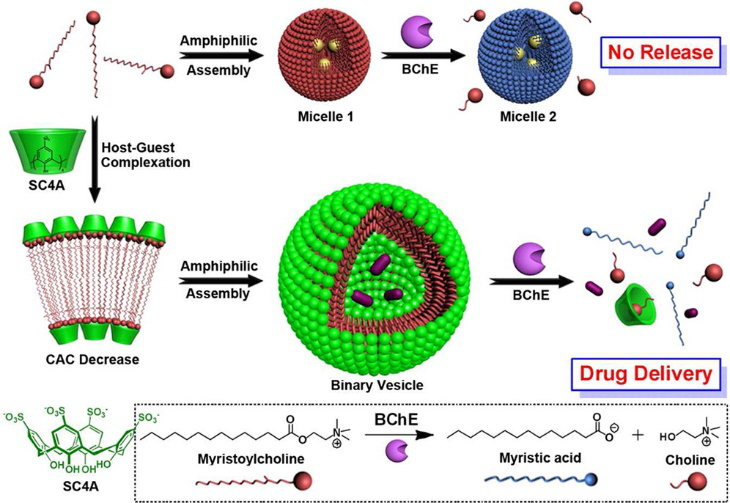
\includegraphics[width= 0.55\textwidth]{Figure/Ch1-SC4A}\\
%        \caption{肉豆蔻酰胆碱在SC4A空白及存在下的两亲自组装示意图}
%    \end{figure}
%    \end{backmatter}
    %%%%%%%%%%%%%%%%%%%%%%%%%%%%%%%%%%%%%%%%%%%%%%%%%%%%%%%%%%%%%%%%%%%%%%%%%%%%%%%
\end{document}